\chapter[Chapitre 3 : Réalisation et tests]{Chapitre 3 : Réalisation\\et tests}
\begin{spacing}{1.2}
\minitoc
\thispagestyle{MyStyle}
\end{spacing}
\clearpage

% Helper : inclut la capture d'écran si le fichier existe (dossier screenshoot/),
% sinon affiche un cadre « à insérer » pour que le document compile quand même.
% Usage : \screenshot{nom-fichier.JPG}{Légende courte du contenu}
\providecommand{\screenshot}[2]{%
  \IfFileExists{../screenshoot/#1}{%
    \includegraphics[width=0.9\textwidth,keepaspectratio]{../screenshoot/#1}%
  }{%
    \fbox{\parbox[c][4.5cm][c]{0.9\textwidth}{\centering\itshape
      Capture d'écran à insérer~: #2\\[4pt]
      \normalfont\small(fichier attendu~: \texttt{screenshoot/#1})}}%
  }%
}

% ─────────────────────────────────────────────────────────────────────────────
\section{Introduction}

Ce chapitre détaille la mise en œuvre concrète de la plateforme NextHire ainsi que les
stratégies de tests appliquées pour valider sa correction et ses performances. La présentation
suit la structure en couches du système : en commençant par l'environnement de développement,
puis en couvrant le backend Node.js et sa couche de persistance, les micro-services Python
d'intelligence artificielle, le moteur de dialogue, le pipeline de détection d'intégrité et
enfin l'application web cliente. La plateforme est entièrement accessible via navigateur :
un front-end React unique sert aussi bien les candidats que les recruteurs, qui disposent
chacun d'un espace dédié au sein de la même application. Le chapitre se conclut par
l'approche de tests adoptée et les résultats obtenus à l'issue des évaluations unitaires,
d'intégration et de bout en bout.

% ─────────────────────────────────────────────────────────────────────────────
\section{Environnement de développement}

\subsection{Outils et technologies utilisés}

Le tableau~\ref{tab:dev-tools} recense les principaux outils de développement utilisés tout
au long du projet.

\begin{table}[H]
  \centering
  \footnotesize
  \renewcommand{\arraystretch}{1.35}
  \setlength{\tabcolsep}{5pt}
  \begin{tabularx}{\textwidth}{|>{\raggedright\arraybackslash}p{3.8cm}|>{\centering\arraybackslash}p{2.2cm}|>{\raggedright\arraybackslash}X|}
    \hline
    \rowcolor{blue!10}
    \textbf{Outil} & \textbf{Version} & \textbf{Rôle} \\
    \hline
    Visual Studio Code & 1.95 & Éditeur de code principal \\
    \hline
    Docker Desktop & 29.5.2 & Orchestration locale des conteneurs \\
    \hline
    Git & 2.54.0 & Gestion de version \\
    \hline
    GitHub & & Dépôt distant et intégration continue \\
    \hline
    Node.js & 26.2.0 & Environnement d'exécution JavaScript (BFF) \\
    \hline
    npm & 11.13.0 & Gestion des paquets Node.js \\
    \hline
    Python & 3.12 & Environnement des micro-services IA \\
    \hline
    pip / venv & 23.x & Gestion des paquets Python et environnements virtuels \\
    \hline
    Postman & & Tests manuels des API REST \\
    \hline
    Groq API & & Inférence LLM cloud (\texttt{openai/gpt-oss-120b}) \\
    \hline
    NVIDIA NIM & & Analyse post-entretien (pipeline LangGraph, \texttt{meta/llama-3.3-70b-instruct}) \\
    \hline
    Google OAuth 2.0 & & Authentification sociale et API Google Calendar \\
    \hline
    MongoDB Compass & & Interface graphique de gestion de la base de données \\
    \hline
  \end{tabularx}
  \caption{Outils de développement et versions utilisés dans le projet NextHire.}
  \label{tab:dev-tools}
\end{table}

\subsection{Organisation du projet}

Le projet est organisé sous la forme d'un monodépôt (\textit{monorepo}) dont la racine
est le répertoire \texttt{ai-recruiter-platform}. Le code source est réparti en deux
grandes branches : \texttt{Backend/} regroupe l'ensemble des services serveur, et
\texttt{Frontend/} contient l'application web React. Chaque service dispose de son propre
manifeste de dépendances (\texttt{package.json} pour Node.js, \texttt{requirements.txt}
pour Python), ce qui garantit un isolement strict des environnements d'exécution.

\begin{sloppypar}
L'organisation des services dans \texttt{Backend/} est la suivante :
\texttt{server/} (BFF Node.js), \texttt{voice\_engine/} (agent d'entretien et pile audio
Python), \texttt{analysis\_service/} (pipeline LangGraph d'analyse post-entretien),
\texttt{face\_verification\_service/} (vérification d'identité InsightFace),
\texttt{yolo-service/} (détection d'objets YOLOv8n) et \texttt{scheduling/}
(intégration Google Calendar). Les services Python disposent chacun d'un fichier
\texttt{docker-compose.yml} permettant de les lancer de manière isolée.
\end{sloppypar}

Le flux de travail adopte une stratégie Git par branches de fonctionnalité
(\textit{feature-branch workflow}) : chaque nouvelle fonctionnalité ou correction de bogue
est développée sur une branche dédiée, soumise à revue, puis fusionnée dans la branche
principale \texttt{main}. Les variables d'environnement ne sont jamais versionnées ; chaque
service lit sa configuration depuis un fichier \texttt{.env} local au démarrage et échoue
immédiatement avec un message explicite si une variable requise est absente.

\subsection{Environnements d'exécution}

La plateforme a été développée et testée dans deux environnements complémentaires, choisis
en fonction des ressources matérielles requises par chaque service.

\paragraph{a) Machine locale (Windows 10 + Docker Desktop).}
La machine locale sous Windows~10 constitue l'environnement de développement principal.
Docker Desktop y fournit un moteur de conteneurisation natif qui permet de lancer les
services Python dans des conteneurs isolés sans modifier l'environnement système. Le
front-end React et le BFF Node.js s'exécutent quant à eux directement sur la machine hôte,
respectivement sur les ports 5173 (serveur de développement Vite) et 3001 (Express).
MongoDB (port~27017) et Redis (port~6379) tournent également en local et sont accessibles
par l'ensemble des services via les variables d'environnement \texttt{MONGO\_URI} et
\texttt{REDIS\_URL}.

\paragraph{b) Inférence IA via API cloud.}
Les opérations d'inférence coûteuses en ressources GPU, à savoir la génération de texte (LLM
\texttt{openai/gpt-oss-120b} via Groq), la transcription vocale (Faster-Whisper) et l'analyse
post-entretien (\texttt{meta/llama-3.3-70b-instruct} via NVIDIA NIM), sont déléguées à des
API cloud spécialisées (Groq et NVIDIA NIM). Cette approche évite l'installation de modèles
volumineux sur la machine de développement et garantit une latence maîtrisée, indépendamment
des capacités graphiques du poste local.

\paragraph{c) Point d'entrée unique (port 3001).}
Plutôt que d'exposer un port distinct pour chaque service, seul le port du BFF Node.js
(3001) est visible depuis le client. En développement, le proxy Vite redirige
automatiquement les appels \texttt{/api/**} et les connexions WebSocket vers ce port
unique. Le BFF joue ainsi le rôle de passerelle centrale : il vérifie le jeton JWT,
orchestre les appels vers les micro-services Python internes et maintient la connexion
Socket.IO pour les échanges en temps réel, sans que le front-end n'ait connaissance de
l'architecture interne des services.

% ─────────────────────────────────────────────────────────────────────────────
\section{Réalisation du backend}

\subsection{Conception de l'API REST}

Le backend Node.js (Express) expose une API REST organisée selon une convention de nommage
orientée ressources. L'ensemble des points de terminaison est regroupé sous le préfixe
\texttt{/api} et retourne des réponses JSON. Le serveur joue le rôle de point d'entrée unique
(\textit{Backend For Frontend}) : il monte une quinzaine de routeurs Express thématiques,
chacun responsable d'un domaine fonctionnel. Le tableau~\ref{tab:api-groups} récapitule les
principaux groupes de points de terminaison.

\begin{table}[H]
  \centering
  \footnotesize
  \renewcommand{\arraystretch}{1.3}
  \setlength{\tabcolsep}{5pt}
  \begin{tabularx}{\textwidth}{|>{\raggedright\arraybackslash}p{3.6cm}|>{\raggedright\arraybackslash}p{3.4cm}|>{\raggedright\arraybackslash}X|}
    \hline
    \rowcolor{blue!10}
    \textbf{Préfixe} & \textbf{Routeur} & \textbf{Rôle} \\
    \hline
    \texttt{/api/auth}, \texttt{/api/users} & \texttt{userRoute} & Connexion, inscription, OAuth Google, profils candidat et recruteur, enrôlement facial \\
    \hline
    \texttt{/api/jobs} & \texttt{jobRoute} & Gestion des offres d'emploi \\
    \hline
    \texttt{/api/wizard/jobs} & \texttt{jobWizardRoute} & Assistant de création d'offre (Job Wizard) \\
    \hline
    \texttt{/api/interviews} & \texttt{interviewRoute} & Cycle de vie de l'entretien, événements d'intégrité, rapports \\
    \hline
    \texttt{/api/call-rooms} & \texttt{callRoom} + \texttt{mediaRoute} & Sessions d'entretien IA, surveillance vision, enregistrements \\
    \hline
    \texttt{/api/job-rooms} & \texttt{jobInterviewRoom} & Salles d'entretien partageables, comparaison des candidats \\
    \hline
    \texttt{/quiz} & \texttt{quizRoute} & Quiz de présélection et modèles de quiz \\
    \hline
    \texttt{/api/messages} & \texttt{messages} & Messagerie temps réel recruteur / candidat \\
    \hline
    \texttt{/api/recommendations} & \texttt{recommendationRoute} & Recommandation d'offres basée sur le profil \\
    \hline
    \texttt{/api/recruiter/calendar}, \texttt{/api/internal/scheduling} & \texttt{recruiterCalendar}, \texttt{schedulingInternal} & Planification d'entretiens et intégration Google Calendar \\
    \hline
    \texttt{/api/linkedin} & \texttt{linkedinRoute} & Liaison et enrichissement du profil LinkedIn \\
    \hline
  \end{tabularx}
  \caption{Principaux groupes de points de terminaison REST du backend NextHire.}
  \label{tab:api-groups}
\end{table}

La validation des données entrantes est réalisée directement dans les gestionnaires de routes
et au niveau des schémas Mongoose, qui appliquent les contraintes de type, les champs requis,
les valeurs énumérées et l'unicité (par exemple l'adresse courriel). Plusieurs limiteurs de
débit (\texttt{express-rate-limit}), adossés en option à Redis, protègent les points de
terminaison sensibles tels que la génération de quiz par IA et la soumission des réponses.

\subsection{Authentification et autorisation}

L'authentification repose sur les jetons web JSON (JWT). Le déroulement est le suivant :

\begin{enumerate}
  \item Le client envoie une requête \texttt{POST /api/auth/login} avec son adresse courriel
        et son mot de passe.
  \item Le backend recherche l'utilisateur, vérifie le mot de passe haché avec
        \texttt{bcryptjs}, puis génère un JWT signé contenant l'identifiant, l'adresse courriel
        et le rôle de l'utilisateur (\texttt{jwt.sign(\{id, email, role\})}).
  \item Le client transmet ce JWT en tant que jeton \textit{Bearer} dans l'en-tête
        \texttt{Authorization} de toutes les requêtes suivantes.
  \item Le middleware \texttt{verifyToken} valide la signature et la date d'expiration du
        jeton avant de transmettre la requête ; toute requête non authentifiée reçoit une
        réponse \texttt{401}, de sorte que les gestionnaires métier ne traitent jamais de
        trafic anonyme.
  \item Le contrôle d'accès basé sur les rôles est assuré par le middleware
        \texttt{requireEnterprise} : les points de terminaison réservés au recruteur rejettent
        les requêtes au rôle candidat, avec un repli sur une vérification en base pour les
        jetons antérieurs ne portant pas encore le champ \texttt{role}.
\end{enumerate}

L'authentification via Google OAuth~2.0 est proposée comme méthode de connexion alternative.
Elle s'appuie sur la stratégie \texttt{passport-google-oauth20} : après autorisation de
l'utilisateur, le profil Google est récupéré via le \textit{callback}
\texttt{/auth/google/callback}, l'utilisateur est créé ou retrouvé en base, et un JWT
natif de la plateforme lui est délivré. Les jetons d'accès et de rafraîchissement Google sont
conservés pour permettre l'intégration ultérieure avec Google Calendar.

\subsection{Module d'extraction et d'analyse de CV}

Lorsqu'un candidat téléverse son CV, le fichier binaire (PDF ou image) est reçu par le
middleware \texttt{Multer} et stocké sur le système de fichiers local du serveur. L'analyse
est ensuite déléguée à un micro-service Python (Flask, port~5002) dédié, qui transforme un
document non structuré en un profil candidat exploitable par la plateforme.

\subsubsection{Extraction du texte (pipeline à deux niveaux)}

L'extraction du texte suit une stratégie en deux niveaux, choisie selon la nature du document~:

\begin{itemize}
  \item \textbf{Extraction native (PDF textuels).} La bibliothèque \texttt{pdfplumber} extrait
        le texte directement du PDF. Une reconstruction \textit{column-aware} a été développée
        pour traiter les CV sur deux colonnes~: un histogramme des positions horizontales des
        mots détecte l'espace inter-colonnes, puis le texte est recomposé colonne de gauche puis
        colonne de droite, afin d'éviter le mélange de lignes que produit l'ordre de lecture par
        défaut.
  \item \textbf{Reconnaissance optique (OCR) en repli.} Lorsque le texte natif est insuffisant
        (moins de 120~caractères ou de 20~mots) ou que le document est une image, le service
        rasterise chaque page avec \texttt{PyMuPDF} (facteur~2$\times$), puis applique
        \textbf{PaddleOCR} (modèle anglais, correction de l'orientation des lignes de texte)
        pour reconstruire le contenu. Le texte retenu est celui qui maximise la quantité
        d'information extraite.
\end{itemize}

Le texte obtenu est normalisé (suppression du bruit typographique, des artefacts
\texttt{(cid:n)} et des séparateurs) avant la phase d'analyse.

\subsubsection{Analyse et structuration du profil}

Le texte nettoyé est ensuite analysé par un pipeline de traitement du langage naturel combinant
la bibliothèque \texttt{spaCy} (modèle \texttt{en\_core\_web\_sm}) et un ensemble de règles et
d'expressions régulières bilingues (français/anglais). Ce pipeline extrait les champs
structurés du profil~: \texttt{name}, \texttt{email}, \texttt{phone}, \texttt{skills},
\texttt{languages}, \texttt{experience} (titre, entreprise, durée, description) et
\texttt{education}. Les compétences sont reconnues à partir d'un dictionnaire de référence
(\texttt{skills\_list.txt}), puis normalisées (par exemple \texttt{nodejs}~$\rightarrow$~%
\texttt{Node.js}) et filtrées par un validateur qui écarte les faux positifs (mots génériques,
fragments de phrases, encodages corrompus). Un \textbf{détecteur de domaine} classe enfin le
profil parmi neuf familles métier (IA / \textit{Machine Learning}, développement logiciel,
\textit{DevOps} / \textit{Cloud}, cybersécurité, etc.) par pondération des mots-clés rencontrés.

Pour écarter les documents qui ne sont pas des CV, un \textbf{classifieur binaire} valide le
résultat~: un modèle TF-IDF (n-grammes de 1 à 2) couplé à une régression logistique, entraîné
sur un jeu d'exemples étiquetés (CV contre factures, menus, relevés bancaires, etc.), produit
une probabilité d'appartenance à la classe «~CV~». Cette probabilité est combinée à des
heuristiques (présence de coordonnées, densité de mots-clés, présence de sections structurées)
pour accepter ou rejeter le document. Le profil validé est persisté dans le sous-document
\texttt{profile} de l'entité \texttt{User}, où il sert de contexte à l'agent d'entretien et au
moteur de recommandation décrit ci-après.

\subsection{Module de recommandation et de \textit{matching} d'offres}

Le \textit{matching} entre candidats et offres est assuré par un second micro-service Python
(Flask, port~5001) qui implémente une approche hybride combinant similarité sémantique et
recouvrement explicite des compétences.

\subsubsection{Représentation sémantique et indexation}

Chaque offre ouverte est convertie en un texte agrégé (titre, description, compétences,
langues) puis encodée en un vecteur dense de 384~dimensions par le modèle
\textbf{Sentence-Transformers} \texttt{all-MiniLM-L6-v2}. Si la bibliothèque n'est pas
disponible, le service bascule automatiquement sur un encodeur de repli
(\texttt{HashingVectorizer} de scikit-learn, 384~dimensions), ce qui garantit la continuité de
service. Les vecteurs sont normalisés et indexés dans un index \textbf{FAISS}
(\texttt{IndexFlatIP})~: le produit scalaire sur des vecteurs normalisés équivaut à une
similarité cosinus, ce qui permet une recherche des plus proches voisins efficace. L'index est
reconstruit périodiquement (toutes les heures, ou à la demande via un point d'accès dédié).

\subsubsection{Score hybride}

Le profil du candidat (résumé, compétences, langues, expériences) est encodé et normalisé de la
même manière, puis comparé à l'index FAISS pour obtenir un ensemble d'offres candidates avec
leur score sémantique. Le score final combine deux composantes~:
\[
  \text{score} = 0{,}25 \times \text{(similarité sémantique)} + 0{,}75 \times \text{(recouvrement pondéré des compétences)}.
\]
Le recouvrement des compétences est calculé après canonicalisation des intitulés (un
dictionnaire de synonymes ramène par exemple \texttt{js}, \texttt{reactjs} ou \texttt{node} à
leur forme canonique), puis pondéré~: chaque compétence porte un poids reflétant son importance
pour le poste (les technologies cœur comme React ou JavaScript pèsent davantage que des outils
secondaires). Une offre déjà candidatée par le candidat est exclue des résultats, et seules les
offres dont le score dépasse un seuil configurable (0{,}3 par défaut) sont retournées, classées
par pertinence décroissante. Chaque recommandation expose enfin le détail de son score
(part sémantique et part compétences), ce qui rend le \textit{matching} transparent pour le
candidat.

\subsection{Module de gestion des entretiens}

Le cycle de vie d'une session d'entretien est piloté par le routeur \texttt{interviewRoute}
en coordination avec \texttt{callRoom}. Les principaux points de terminaison sont les
suivants :

\begin{itemize}
  \item \texttt{POST /api/call-rooms/create} crée une nouvelle salle d'entretien IA pour
        un candidat et un poste donnés.
  \item \texttt{GET /api/call-rooms/:roomId} retourne le contexte complet de la session
        (profil candidat, exigences du poste, statut) destiné au moteur de dialogue.
  \item \texttt{POST /api/call-rooms/:roomId/vision-monitoring} enregistre un événement
        d'intégrité (vision ou navigateur) avec sa sévérité et ses métadonnées.
  \item \texttt{POST /api/interviews/:interviewId/analyze-video} déclenche le pipeline
        LangGraph d'analyse post-entretien en arrière-plan.
  \item \texttt{GET /api/interviews/:interviewId/final-report} retourne le rapport recruteur
        final (scores pondérés, points forts, lacunes, recommandation d'embauche).
  \item \texttt{GET /api/interviews/:interviewId/integrity-report} retourne le rapport
        d'intégrité agrégé (niveau de risque, violations détectées).
\end{itemize}

% ─────────────────────────────────────────────────────────────────────────────
\section{Réalisation du détecteur de fraude}

\subsection{Architecture du détecteur}

Contrairement à une approche monolithique où l'ensemble de la détection s'exécuterait dans
un unique serveur, NextHire répartit la surveillance d'intégrité sur trois couches
complémentaires, ce qui réduit la charge réseau et préserve la confidentialité (aucune image
brute ne quitte le poste sans nécessité) :

\begin{itemize}
  \item \textbf{Analyse côté client (React).} Le composant \texttt{VisionMonitor} exécute
        directement dans le navigateur le modèle \textit{MediaPipe Face Landmarker}
        (bibliothèque \texttt{@mediapipe/tasks-vision}) à une cadence de 5~images/s. Il assure
        la détection du visage, le contrôle de présence, de centrage, de distance, de
        l'éclairage et de l'attention, sans transmettre la vidéo au serveur.
  \item \textbf{Service de vérification d'identité (Python / Flask).} Le service
        \texttt{face\_verification\_service} encapsule le modèle \textit{InsightFace}
        (\texttt{buffalo\_l}) via ONNXRuntime pour la confrontation d'identité 1:1.
  \item \textbf{Service de détection d'objets (Python / FastAPI).} Le service
        \texttt{yolo-service} encapsule le modèle \textit{YOLOv8n} pour la détection d'objets
        interdits dans le champ de la caméra.
\end{itemize}

Les événements produits par ces trois couches sont transmis au backend Node.js via
Socket.IO et REST, puis horodatés et enregistrés dans le document \texttt{CallRoom} de la
session. Par conception, ces détecteurs ne produisent que des constats objectifs (présence
d'objet, nombre de personnes, identité) : ils n'infèrent ni émotion, ni stress, ni
caractéristique personnelle, et le recruteur demeure le seul décideur final.

\subsection{Modules de détection}

\subsubsection{Détection du visage et de visages multiples}

Le \texttt{VisionMonitor} client s'appuie sur \textit{MediaPipe Face Landmarker} pour
localiser le visage du candidat sur chaque trame. L'absence prolongée de visage déclenche une
violation \texttt{NO\_FACE\_DETECTED}, tandis que la détection de plusieurs visages déclenche
\texttt{MULTIPLE\_FACES\_DETECTED}. En parallèle, la vérification d'identité continue est
confiée au service \textit{InsightFace} : pour chaque trame contrôlée, le service calcule
un \textit{embedding} facial normalisé de 512 dimensions et le compare, par similarité
cosinus, à l'\textit{embedding} de référence enregistré lors de l'inscription. Une similarité
inférieure au seuil de \texttt{0{,}60} signale une discordance d'identité.

\subsubsection{Suivi de l'attention et du cadrage}

À partir des points de repère faciaux fournis par \textit{MediaPipe Face Landmarker}, le
moniteur évalue en continu plusieurs indicateurs géométriques : le centrage du visage dans le
cadre (tolérances de \texttt{0{,}18} en horizontal et \texttt{0{,}20} en vertical), la
distance à la caméra estimée par le ratio surfacique du visage (plage acceptable de
\texttt{0{,}12} à \texttt{0{,}55}), la qualité de l'éclairage (luminance moyenne) et la
netteté de l'image. Une orientation du regard hors de l'écran maintenue au-delà du seuil
temporel déclenche une violation \texttt{LOOKING\_AWAY\_LONG}, et un visage mal cadré ou trop
éloigné produit respectivement \texttt{FACE\_NOT\_CENTERED} et \texttt{BAD\_FACE\_DISTANCE}.

\subsubsection{Détection d'objets}

Le service \texttt{yolo-service} charge le modèle pré-entraîné \textit{YOLOv8n} et restreint
les détections aux classes COCO pertinentes : téléphone (\texttt{cell phone}, 67), livre
(\texttt{book}, 73), ordinateur portable (\texttt{laptop}, 63), écran (\texttt{tv}, 62) et
personne (\texttt{person}, 0). Des seuils de confiance spécifiques par classe sont appliqués
(\texttt{0{,}30} pour le téléphone et le livre, \texttt{0{,}50} pour les écrans) afin de
limiter les faux positifs sur des trames webcam de 640~pixels. Chaque détection retenue est
convertie en violation typée : \texttt{PHONE\_VISIBLE}, \texttt{REFERENCE\_MATERIAL\_VISIBLE},
\texttt{SCREEN\_DEVICE\_VISIBLE}, \texttt{MULTIPLE\_PEOPLE} ou \texttt{NO\_PERSON\_VISIBLE}.

\subsection{Production du rapport d'intégrité}

À la fin de la session, le backend Node.js agrège l'ensemble des violations enregistrées via
la fonction \texttt{buildVisionReport()}. Chaque type de violation contribue à un score de
risque pondéré : par exemple, la présence de plusieurs personnes ou de plusieurs visages
pèse 25~points, un téléphone ou un écran détecté 15~points, une absence du candidat 15~points,
et un changement d'onglet 10~points. Le score cumulé est plafonné à 100, puis traduit en un
niveau de risque (\textit{low}, \textit{medium}, \textit{high} ou \textit{critical})
accompagné d'une recommandation textuelle. Le rapport d'intégrité ainsi constitué est
persisté dans le document \texttt{CallRoom} et présenté au recruteur dans son tableau de bord
sous forme de chronologie d'événements et de cartes de synthèse (figure~\ref{fig:integrity-report}),
sans génération de fichier PDF externe.

\begin{figure}[H]
  \centering
  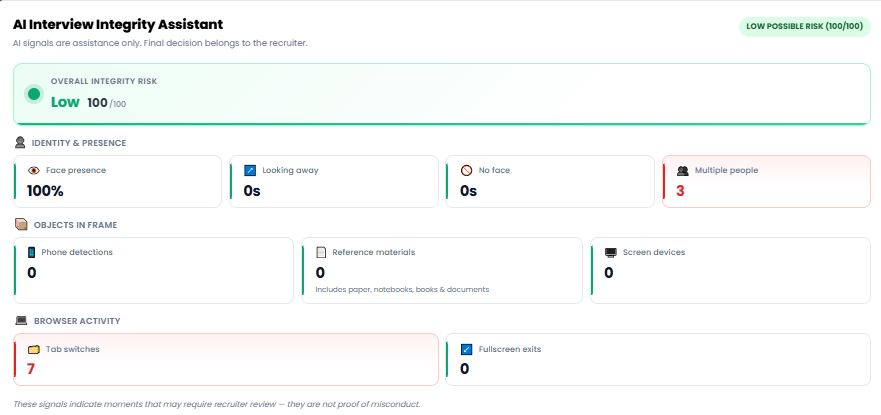
\includegraphics[width=0.9\textwidth,keepaspectratio]{../screenshoot/integrity.JPG}
  \caption{Exemple de rapport d'intégrité présenté au recruteur dans le tableau de bord NextHire.}
  \label{fig:integrity-report}
\end{figure}

\subsection{Analyse multimodale post-entretien}

Distincte du détecteur de fraude, dont les signaux restent de simples constats objectifs, l'analyse multimodale post-entretien enrichit l'évaluation du candidat par deux sources complémentaires de signal affectif. Pour l'\textbf{émotion faciale}, le service d'analyse s'appuie sur \textit{Py-Feat}, une boîte à outils entraînée sur le corpus \textit{AffectNet} d'images de visages réels. Plutôt que de prédire directement des probabilités d'émotion, souvent peu fiables, Py-Feat extrait les \textit{unités d'action faciales} (FACS, \textit{Facial Action Coding System}) — mouvements élémentaires des muscles du visage — à partir desquelles sont dérivés les états émotionnels normalisés (joie, surprise, neutralité, etc.). Pour le \textbf{sentiment vocal}, la réponse du candidat, une fois transcrite par Faster-Whisper, est soumise à un modèle de classification de séquences fondé sur \textit{RoBERTa} (\texttt{cardiffnlp/twitter-roberta-base-sentiment-latest}), qui restitue une polarité (positif, neutre, négatif) assortie d'un score de confiance.

Il importe de souligner que ces signaux multimodaux sont traités comme des \textit{indices complémentaires}, destinés à contextualiser la prestation du candidat (par exemple, moduler le comportement de l'agent en cas de stress détecté), et non comme un déterminant de la décision. Aucune note d'embauche n'est calculée à partir de l'émotion ou du sentiment : l'évaluation des compétences repose sur le contenu des réponses, et la décision finale demeure une prérogative exclusive du recruteur humain. Ce parti pris répond aux préoccupations éthiques bien documentées concernant l'inférence d'états affectifs en contexte de recrutement.

% ─────────────────────────────────────────────────────────────────────────────
\section{Réalisation de l'application web}

\subsection{Aperçu de l'interface utilisateur}

L'application cliente de NextHire est une application web monopage développée avec React~19
et empaquetée par Vite. Contrairement à une application de bureau, elle s'exécute
intégralement dans le navigateur et ne nécessite aucune installation. Le routage est assuré
par \texttt{react-router-dom}, qui distingue les espaces propres à chaque rôle : les écrans
candidat (profil, planification, salle d'entretien) et les écrans recruteur (espace
entreprise, salles d'entretien, comparaison des candidats), en plus d'un tableau de bord
d'administration.

La protection des routes et la gestion de session reposent sur un contexte React partagé,
\texttt{AuthContext}. À la connexion, le jeton JWT est conservé dans le \texttt{localStorage}
du navigateur, puis attaché à chaque appel au backend sous la forme d'un en-tête
\texttt{Authorization: Bearer <token>}. En cas de réponse signalant un jeton expiré ou
invalide, le contexte déconnecte l'utilisateur et le redirige vers la page de connexion. La
communication en temps réel (entretien, messagerie, alertes d'intégrité) s'appuie quant à
elle sur le client \texttt{socket.io-client}.

\subsection{Écrans candidat}

\subsubsection{Profil et tableau de bord candidat}

L'écran de profil candidat (route \texttt{/candidate/:id}) centralise les informations du
candidat : photo de profil vérifiée pour le contrôle d'identité, compétences, langues,
expériences et CV téléversé. Il présente également les candidatures soumises et les offres
recommandées par le moteur de recommandation. Un indicateur de complétude du profil incite
le candidat à compléter ses informations et à téléverser son CV, étape nécessaire avant de
postuler (figure~\ref{fig:candidate-profile}).

\begin{figure}[H]
  \centering
  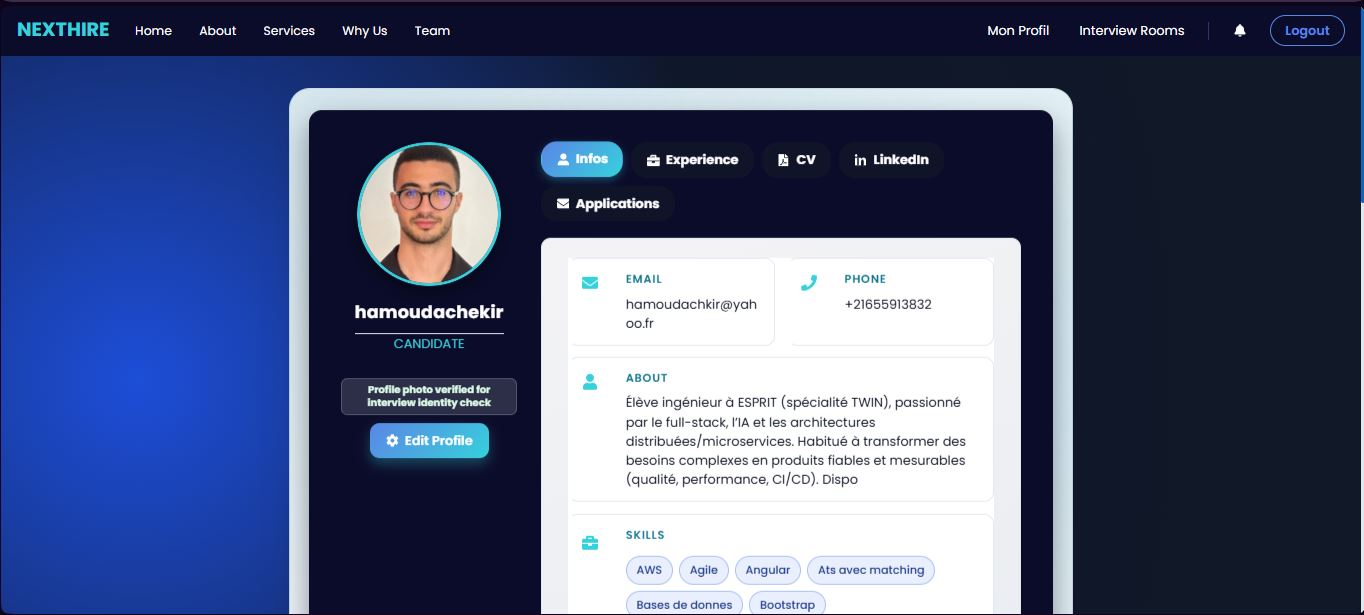
\includegraphics[width=0.48\textwidth,keepaspectratio]{images/profile1.JPG}\hfill
  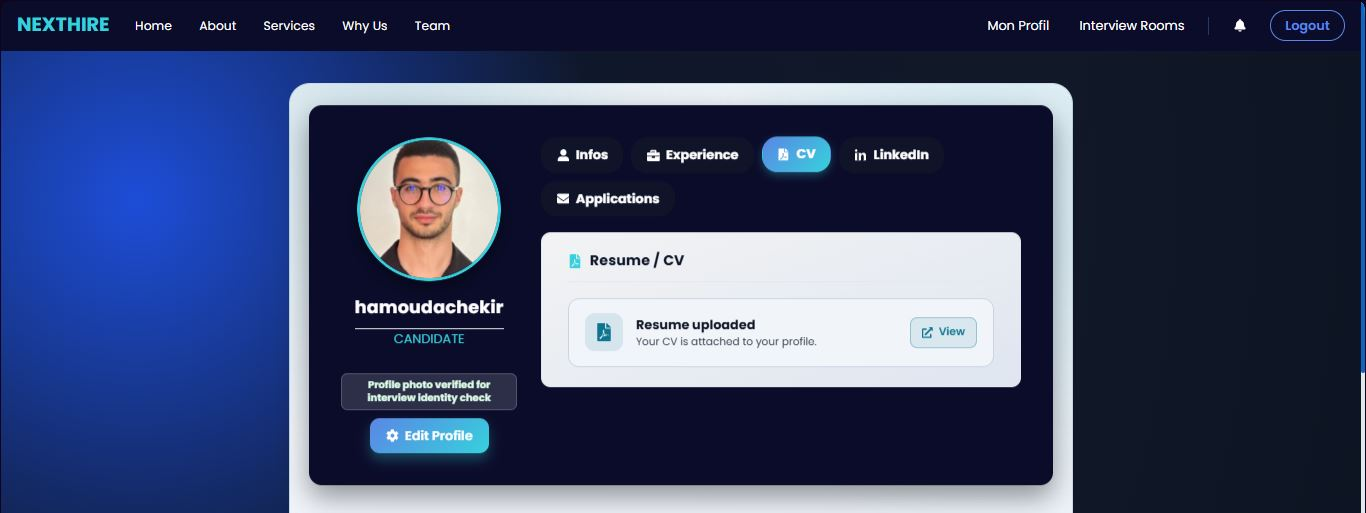
\includegraphics[width=0.48\textwidth,keepaspectratio]{images/profile2.JPG}\\[6pt]
  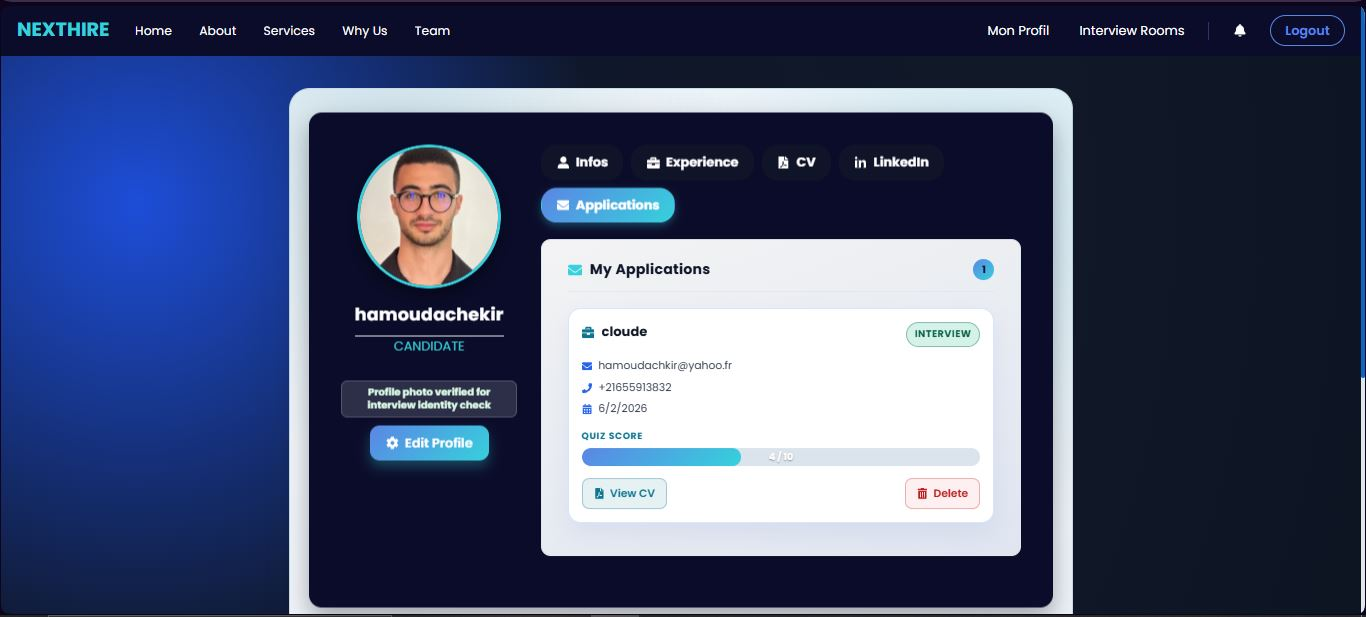
\includegraphics[width=0.6\textwidth,keepaspectratio]{images/profile3.JPG}
  \caption{Écran de profil et tableau de bord du candidat.}
  \label{fig:candidate-profile}
\end{figure}

\subsubsection{Page d'accueil et recommandation d'offres}

Dès sa connexion, le candidat arrive sur une page d'accueil qui met en avant une liste
d'offres recommandées personnalisées (figure~\ref{fig:candidate-home}). Le \textit{front-end}
React interroge la route \texttt{GET /recommendation/for-user}, qui relaie la requête au
micro-service de recommandation Python (port~5001) décrit au chapitre~2. Pour la page
d'accueil, le backend demande jusqu'à dix offres (\texttt{top\_k}~=~10) avec un seuil de
similarité abaissé à $0{,}2$ (au lieu de $0{,}3$ par défaut), afin d'élargir l'éventail
d'offres proposées au candidat.

Chaque offre est restituée avec son score de correspondance (\texttt{match\_score}) issu du
score hybride, et les informations de l'entreprise (nom, logo) sont jointes en une seule
requête à la base de données pour enrichir l'affichage. Les offres auxquelles le candidat a
déjà postulé sont automatiquement écartées par le service de recommandation. Le candidat peut
alors consulter le détail d'une offre et postuler directement depuis cette page. Pour préserver
la robustesse de l'interface, l'API se comporte de façon dégradée : si le service de
recommandation est momentanément indisponible, elle renvoie une liste vide plutôt qu'une
erreur, et la page d'accueil reste fonctionnelle.

\begin{figure}[H]
  \centering
  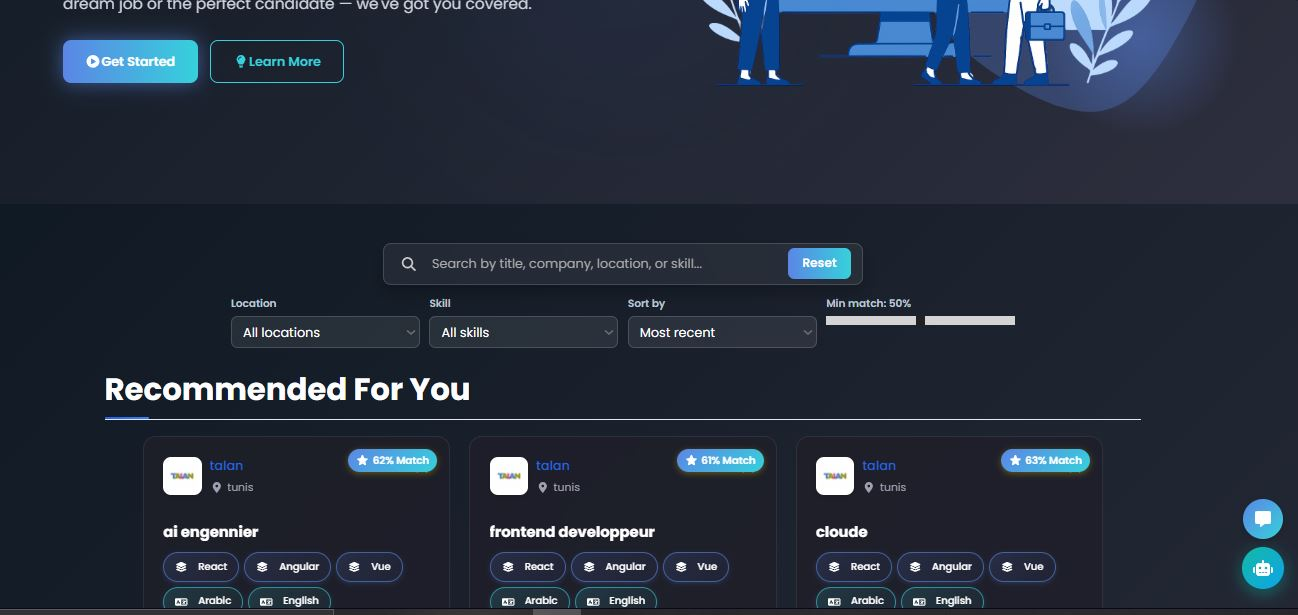
\includegraphics[width=0.9\textwidth,keepaspectratio]{images/home.JPG}
  \caption{Page d'accueil candidat avec les offres recommandées.}
  \label{fig:candidate-home}
\end{figure}

\subsubsection{Salles d'entretien disponibles}

Le candidat dispose d'un écran listant les salles d'entretien disponibles auxquelles il peut
se joindre (figure~\ref{fig:available-rooms}), alimenté par la route
\texttt{GET /api/call-rooms/available}. Cette liste se met à jour en temps réel grâce à
Socket.IO : lorsqu'un recruteur ouvre une nouvelle salle, celle-ci apparaît instantanément
chez les candidats concernés, et toute salle clôturée ou déjà démarrée en est retirée
automatiquement. Pour rejoindre un entretien, le candidat envoie une demande
(\texttt{request-join}) puis attend la confirmation du recruteur ; dès que celle-ci est reçue,
il est redirigé automatiquement vers la salle d'entretien. Un mécanisme de secours par
interrogation périodique assure cette redirection même si l'événement temps réel venait à être
manqué.

\begin{figure}[H]
  \centering
  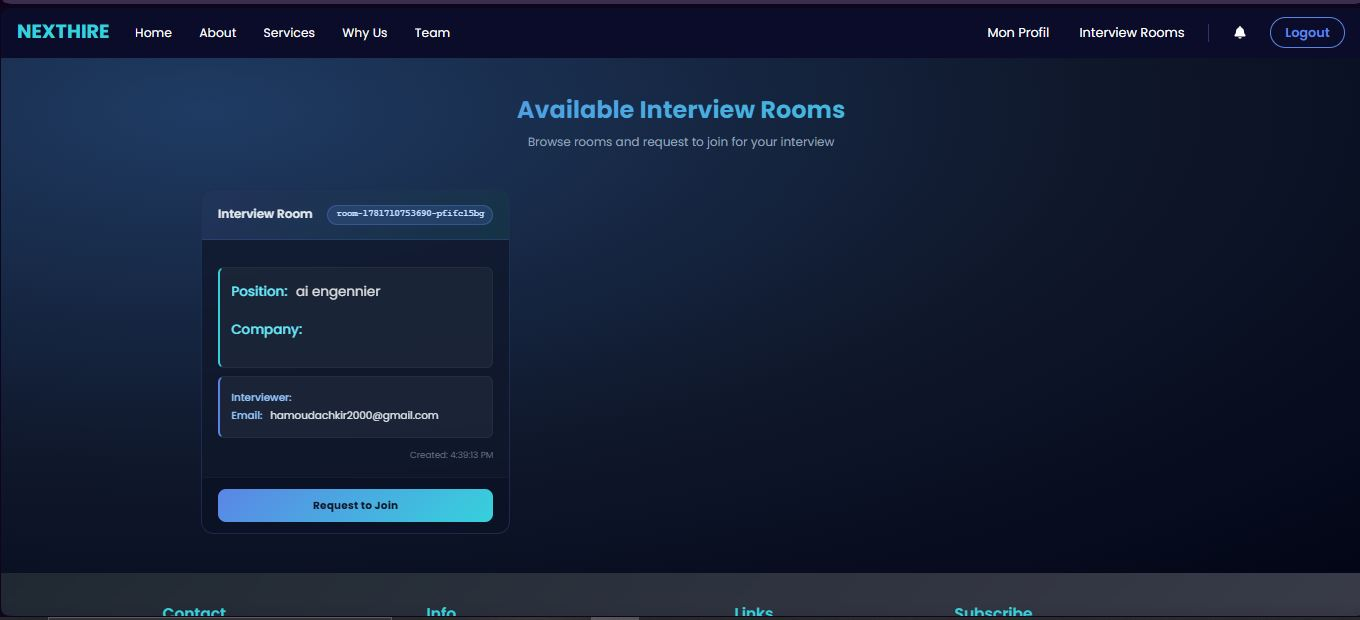
\includegraphics[width=0.9\textwidth,keepaspectratio]{images/available-room.JPG}
  \caption{Liste des salles d'entretien disponibles pour le candidat.}
  \label{fig:available-rooms}
\end{figure}

\subsubsection{Écran de vérification pré-entretien}

Avant d'accéder à la salle d'entretien, le candidat passe par un écran de vérification
(composants \texttt{FaceVerification} et \texttt{VisionMonitor}). Celui-ci contrôle d'abord
les autorisations de la caméra et du microphone via l'API \textit{Permissions} du navigateur,
puis exécute un précontrôle en temps réel : présence et centrage du visage, qualité de
l'éclairage et unicité du visage dans le cadre. En parallèle, la vérification d'identité
faciale confronte l'image en direct à l'\textit{embedding} de référence du candidat
(InsightFace). Le candidat ne peut rejoindre l'entretien en direct que lorsque l'ensemble de
ces contrôles est validé (figure~\ref{fig:pre-interview}).

\begin{figure}[H]
  \centering
  \screenshot{pre-interview-verification.JPG}{Vérification caméra, micro et identité faciale}
  \caption{Écran de vérification pré-entretien.}
  \label{fig:pre-interview}
\end{figure}

\subsubsection{Écran d'entretien avec avatar 3D}

L'écran principal d'entretien (route \texttt{/call-room/:roomId}, composant
\texttt{CallRoomActive}) constitue le cœur de l'interaction en direct avec le candidat. Il
affiche un avatar~3D animé, rendu avec \texttt{three.js} et \texttt{react-three-fiber}, qui
incarne l'assistante d'entretien \textit{Nour} : l'avatar énonce vocalement les questions et
synchronise le mouvement de ses lèvres avec l'audio (\textit{lip-sync}). Un panneau de
transcription en temps réel restitue au candidat ses propres réponses au fur et à mesure de
la conversation, tandis que la surveillance d'intégrité (vision et identité) s'exécute en
arrière-plan tout au long de la session (figure~\ref{fig:interview-avatar}).

\begin{figure}[H]
  \centering
  \screenshot{interview-avatar.JPG}{Salle d'entretien avec avatar 3D et transcription}
  \caption{Écran d'entretien avec avatar 3D (assistante \textit{Nour}).}
  \label{fig:interview-avatar}
\end{figure}

\subsection{Écrans recruteur}

\subsubsection{Tableau de bord recruteur}

L'espace recruteur (route \texttt{/entreprise/:id}, composant \texttt{EntrepriseProfile})
présente les offres d'emploi publiées par l'entreprise, le nombre de candidatures par offre
et la liste des candidats associés. Le recruteur peut y créer ou modifier une offre grâce à
l'assistant de création (\textit{Job Wizard}), suivre l'avancement des candidatures et
accéder au profil de chaque candidat (figure~\ref{fig:recruiter-dashboard}).

\begin{figure}[H]
  \centering
  \screenshot{recruiter-dashboard.JPG}{Espace entreprise : offres et candidatures}
  \caption{Tableau de bord recruteur avec vue des offres et des candidatures.}
  \label{fig:recruiter-dashboard}
\end{figure}

\subsubsection{Salles d'entretien et comparaison des candidats}

L'écran des salles d'entretien (route \texttt{/entreprise/:entrepriseId/interview-rooms},
composant \texttt{JobInterviewRooms}) permet au recruteur de créer une salle partageable
associée à un poste et de suivre les sessions des candidats. À l'issue de plusieurs entretiens,
l'écran de comparaison (\texttt{CandidateComparison}) classe les candidats selon un score
composite (technique, communication, résolution de problèmes, adéquation RH) et restitue le
résumé exécutif ainsi que la recommandation d'embauche produite par l'agent d'analyse
(figure~\ref{fig:candidate-comparison}).
Ce score composite de classement ---~score global, adéquation au poste, couverture des compétences, confiance du rapport et pénalité de biais~--- est distinct de la grille d'évaluation par question utilisée pendant l'entretien, qui repose sur le score adaptatif IRT-lite~$\theta$ mis à jour à chaque tour. Les deux grilles répondent à des objectifs complémentaires : l'une note la qualité de chaque réponse en temps réel, l'autre agrège les résultats de l'entretien pour permettre la comparaison entre candidats.

\begin{figure}[H]
  \centering
  \screenshot{candidate-comparison.JPG}{Classement et comparaison des candidats}
  \caption{Écran de comparaison et de classement des candidats pour un poste.}
  \label{fig:candidate-comparison}
\end{figure}

\subsubsection{Écran de revue d'entretien}

L'écran de revue permet au recruteur d'examiner en détail un entretien terminé. Il affiche
en en-tête le nom du candidat, le poste concerné et la date de l'entretien. En dessous, une
transcription interactive liste chaque question posée par l'agent, la réponse du candidat,
le score et la justification produits par l'évaluation pondérée, ainsi que les éventuelles
violations détectées. Le rapport d'intégrité associé (niveau de risque, chronologie des
événements, recommandation) est présenté en regard, sans génération de fichier PDF externe
(figure~\ref{fig:interview-review}).

\begin{figure}[H]
  \centering
  \screenshot{interview-review.JPG}{Revue d'entretien : transcription, scores, intégrité}
  \caption{Écran de revue d'entretien côté recruteur.}
  \label{fig:interview-review}
\end{figure}

% ─────────────────────────────────────────────────────────────────────────────
\section{Tableau de bord administrateur}

NextHire intègre un espace d'administration séparé, accessible sous le préfixe
\texttt{/dashboard}, protégé par un gardien de route dédié (\texttt{AdminProtectedRoute}).
Cet espace offre une vue centralisée de l'ensemble de la plateforme sans être lié à un
compte recruteur particulier.

\subsection{Vue d'ensemble et indicateurs clés}

La page d'accueil du tableau de bord agrège en temps réel les données de la plateforme via
l'endpoint \texttt{GET /api/admin/stats}. Six cartes d'indicateurs sont affichées en grille~:
le nombre de candidats inscrits, d'entreprises enregistrées, d'offres publiées, de
candidatures reçues, d'entretiens créés et d'entretiens planifiés. Deux graphiques complètent
cette vue~: un diagramme en anneau (\textit{donut chart}) représentant la répartition des
offres par statut, et un histogramme miniature indiquant l'évolution des candidatures dans
le temps. Un second diagramme en anneau distingue les entretiens confirmés des entretiens
en attente de planification (figure~\ref{fig:admin-dashboard}).

\begin{figure}[H]
  \centering
  \screenshot{admin-dashboard.JPG}{Tableau de bord admin : KPI, graphiques, listes récentes}
  \caption{Tableau de bord administrateur~: indicateurs en temps réel et graphiques d'activité.}
  \label{fig:admin-dashboard}
\end{figure}

\subsection{Gestion des entités}

La barre de navigation latérale donne accès à cinq sections de gestion~:

\begin{itemize}
  \item \textbf{Candidates} (\texttt{/dashboard/manage-candidates}) : liste paginée des
        candidats avec leurs informations de profil et leur statut de vérification.
  \item \textbf{Companies} (\texttt{/dashboard/manage-employees}) : gestion des comptes
        entreprise et de leurs informations administratives.
  \item \textbf{Jobs} (\texttt{/dashboard/jobs}) : consultation de toutes les offres publiées
        sur la plateforme, indépendamment de l'entreprise propriétaire.
  \item \textbf{Calendar} (\texttt{/dashboard/calendar}) : vue calendrier des entretiens
        planifiés sur l'ensemble des salles actives.
  \item \textbf{Settings} (\texttt{/dashboard/settings}) : paramètres globaux de la
        plateforme.
\end{itemize}

Cet espace d'administration permet de superviser l'activité de la plateforme et de
corriger d'éventuelles anomalies sans intervenir directement dans les comptes utilisateurs,
conformément au principe de séparation des responsabilités retenu lors de la conception.

% ─────────────────────────────────────────────────────────────────────────────
\section{Sécurité et conformité}

La sécurité de NextHire repose sur une stratégie de défense en profondeur : plusieurs couches
indépendantes couvrent l'identité, l'autorisation, la protection contre les abus, l'intégrité
de l'entretien et la conformité réglementaire. Cette section consolide l'ensemble des mécanismes
implémentés dans la plateforme.

\subsection{Authentification}

\subsubsection{Jetons JWT}

L'authentification repose sur des jetons web JSON (\textit{JSON Web Tokens}, JWT) signés en
HS256 à partir d'un secret applicatif stocké dans les variables d'environnement. Le flux est le
suivant : lors de la connexion, le mot de passe fourni est vérifié contre le condensé
\texttt{bcryptjs} stocké en base (facteur de coût configurable, défaut 10) ; en cas de succès,
un JWT portant les champs \texttt{\{id, email, role\}} est signé et renvoyé au client. Toutes
les requêtes suivantes transmettent ce jeton en tant que \textit{Bearer token} dans l'en-tête
\texttt{Authorization}. Le middleware \texttt{verifyToken} valide la signature et la date
d'expiration avant tout traitement métier ; tout jeton absent, malformé ou expiré produit
systématiquement une réponse \texttt{HTTP 401}, de sorte que les gestionnaires de routes ne
traitent jamais de trafic non authentifié.

\subsubsection{Authentification sociale -- Google OAuth 2.0}

Une méthode de connexion alternative est proposée via la stratégie \texttt{passport-google-oauth20}.
Après autorisation de l'utilisateur sur le consentement Google, le profil est récupéré via le
\textit{callback} \texttt{/auth/google/callback} ; l'utilisateur est créé ou récupéré en base,
et un JWT natif NextHire lui est délivré. Les jetons d'accès et de rafraîchissement Google sont
conservés exclusivement pour permettre l'intégration avec Google Calendar ; ils ne sont pas
exposés au client.

\subsection{Autorisation par rôles -- RBAC}

Le contrôle d'accès basé sur les rôles est assuré par le middleware \texttt{requireEnterprise},
appliqué à tous les points de terminaison réservés aux recruteurs. Son comportement suit deux
chemins :

\begin{itemize}
  \item \textbf{Chemin rapide.} Si le JWT porte le champ \texttt{role = 'ENTERPRISE'},
        l'accès est accordé immédiatement sans requête base de données.
  \item \textbf{Repli base de données.} Pour les jetons antérieurs ne portant pas encore
        le champ \texttt{role} (compatibilité ascendante), le middleware interroge MongoDB
        (\texttt{User.findById().select('role').lean()}) et met à jour \texttt{req.user.role}
        en mémoire pour les middlewares aval.
\end{itemize}

Toute requête dont le rôle ne correspond pas à \texttt{ENTERPRISE} reçoit une réponse
\texttt{HTTP 403} avant d'atteindre la logique métier. Cette approche \textit{fail-closed}
garantit qu'une erreur de configuration (jeton sans rôle, base indisponible) bloque l'accès
plutôt que de l'autoriser par défaut.

\subsection{Limitation de débit}

Deux limiteurs de débit indépendants, fondés sur \texttt{express-rate-limit}, protègent les
points de terminaison à risque élevé.

\begin{table}[H]
  \centering
  \footnotesize
  \renewcommand{\arraystretch}{1.3}
  \begin{tabularx}{\textwidth}{|>{\raggedright\arraybackslash}p{3.5cm}|>{\raggedright\arraybackslash}X|>{\raggedright\arraybackslash}p{2.8cm}|}
    \hline
    \textbf{Limiteur} & \textbf{Règle} & \textbf{Clé de comptage} \\
    \hline
    \texttt{aiGenerationRateLimiter} & 10 requêtes par minute par utilisateur (configurable via \texttt{AI\_GENERATION\_MAX\_PER\_MINUTE}) & \texttt{req.user.\_id} (repli sur IP) \\
    \hline
    \texttt{quizRateLimiter} & 3 soumissions par tranche de 24\,h par couple candidat\,+\,offre (configurable via \texttt{QUIZ\_MAX\_ATTEMPTS\_PER\_DAY}) & \texttt{candidateId-jobId} (repli sur IP) \\
    \hline
  \end{tabularx}
  \caption{Limiteurs de débit de la plateforme NextHire.}
  \label{tab:rate-limiters}
\end{table}

Les deux limiteurs partagent la même architecture de stockage : en développement, un compteur
en mémoire est utilisé ; en production, un stockage Redis (\texttt{rate-limit-redis}) est activé
par la variable d'environnement \texttt{QUIZ\_RATE\_LIMIT\_USE\_REDIS=true}. En cas d'échec de
connexion à Redis, le système se replie automatiquement sur le compteur en mémoire avec un
avertissement journalisé. Les requêtes ayant échoué à la validation (\textit{skipFailedRequests})
ne sont pas décomptées du quota.

\subsection{Vérification faciale -- comportement \textit{fail-closed}}

Avant chaque entretien, un module de vérification d'identité compare l'image capturée en temps
réel par la webcam à la photo de profil enregistrée lors de l'enrôlement. La comparaison repose
sur un vecteur d'embedding de 512 dimensions calculé par InsightFace (modèle \texttt{buffalo\_l})
et une distance cosinus. Le comportement est \textit{fail-closed} : toute condition anormale
bloque l'accès à la salle d'entretien plutôt que de le laisser passer.

\begin{itemize}
  \item \textbf{Service indisponible.} Si le micro-service de vérification faciale ne répond
        pas, la décision de démarrage est refusée (\texttt{status: 'failed',
        reason: 'face\_verification\_disabled'}).
  \item \textbf{Candidat non enrôlé.} Si aucun profil facial n'a été préalablement enregistré
        pour le candidat, l'accès est bloqué et un événement d'audit
        \texttt{NOT\_ENROLLED} est enregistré.
  \item \textbf{Similarité insuffisante.} Si la distance cosinus entre les deux embeddings
        dépasse le seuil $\tau = 0{,}60$, la vérification échoue et l'événement est journalisé
        avec les métadonnées d'audit (nombre de trames valides, score moyen).
\end{itemize}

La confidentialité est préservée par conception : aucune image brute ne quitte le poste du
candidat. Seuls les vecteurs d'embedding sont transmis via l'API REST interne, ce qui limite
l'exposition des données biométriques au strict nécessaire.

\subsection{Conformité RGPD}

La plateforme a été conçue pour respecter les principes du Règlement Général sur la Protection
des Données :

\begin{itemize}
  \item \textbf{Consentement explicite.} Le candidat est informé, lors de l'enrôlement facial
        et avant le démarrage de l'entretien, que sa webcam et son microphone sont activés
        à des fins d'évaluation. L'entretien ne peut commencer sans validation de cette étape.
  \item \textbf{Minimisation des données biométriques.} Comme décrit à la section précédente,
        seuls les embeddings (vecteurs de 512 dimensions) sont transmis ; les images brutes ne
        quittent pas le poste du candidat.
  \item \textbf{Décision finale humaine.} Le rapport post-entretien généré par l'IA fournit
        des scores, des points forts et des lacunes, et se conclut par une recommandation
        (\textit{Strong Hire / Hire / No Hire / Strong No Hire}) ; la décision finale
        d'acceptation ou de refus reste une action explicite du recruteur, tracée en base de
        données. L'IA n'embauche pas : elle informe.
  \item \textbf{Chiffrement des données en transit.} Toutes les communications entre le
        navigateur et les services backend sont protégées par TLS (HTTPS). Les mots de
        passe ne sont jamais stockés en clair : seul le condensé \texttt{bcryptjs} est
        persisté.
\end{itemize}

% ─────────────────────────────────────────────────────────────────────────────
\section{Tests}

\subsection{Stratégie de tests et outillage}

La validation de NextHire suit le principe de la pyramide des tests : une base large de tests
unitaires rapides et isolés, un étage intermédiaire de tests d'intégration qui éprouvent les
frontières entre composants, et un sommet plus étroit de tests de bout en bout et de validation
système. Les dépendances lourdes (modèles PyTorch, Faster-Whisper, YOLO, accès réseau aux
API Groq et Edge TTS, MongoDB, Redis) sont remplacées par des doublures
(\textit{stubs} enregistrés dans \texttt{sys.modules} côté Python, données factices côté
Node.js), de sorte que la suite s'exécute en quelques secondes, sans GPU ni clé d'API. Les
tests qui exigent une infrastructure réelle sont isolés et ignorés automatiquement lorsque
celle-ci est absente. Le tableau~\ref{tab:test-frameworks} récapitule les frameworks employés
par service et par niveau.

\begin{table}[H]
  \centering
  \footnotesize
  \renewcommand{\arraystretch}{1.3}
  \setlength{\tabcolsep}{5pt}
  \begin{tabularx}{\textwidth}{|>{\raggedright\arraybackslash}p{3.4cm}|>{\raggedright\arraybackslash}p{2.3cm}|>{\raggedright\arraybackslash}p{3.0cm}|>{\raggedright\arraybackslash}X|}
    \hline
    \rowcolor{blue!10}
    \textbf{Service} & \textbf{Niveau} & \textbf{Framework} & \textbf{Fichier représentatif} \\
    \hline
    Backend Node.js & Unitaire & \texttt{node:assert} & \texttt{faceVerifyDecision.test.js} \\
    \hline
    Moteur d'entretien (\texttt{voice\_engine}) & Unitaire & \texttt{unittest} + stubs & \texttt{test\_interview\_agent\_conversation.py} \\
    \hline
    Service d'analyse (\texttt{analysis\_service}) & Unitaire / intégration & \texttt{pytest} & \texttt{test\_report\_schema.py} \\
    \hline
    Frontend (React) & Bout en bout & Playwright & \texttt{e2e-rh-job-match.spec.js} \\
    \hline
    Système & Validation & Scripts Python & \texttt{tests/} (charge, chaos, ML, intégrité) \\
    \hline
  \end{tabularx}
  \caption{Frameworks de test par service et par niveau.}
  \label{tab:test-frameworks}
\end{table}

\subsection{Tests unitaires}

\subsubsection{Backend Node.js}

Le module décisionnel de la vérification faciale est couvert par un test en
\texttt{node:assert} (\texttt{faceVerifyDecision.test.js}) regroupant 13~assertions. Celles-ci
vérifient le comportement \textit{fail-closed} de la décision de démarrage d'entretien :
la projection de sélection des candidats n'expose jamais l'\textit{embedding} facial parent,
une correspondance stricte n'est validée que lorsque le nombre minimal de trames concordantes
est atteint, et toute configuration ambiguë conduit à un refus plutôt qu'à une autorisation.

\subsubsection{Moteur d'entretien}

Deux modules de tests unitaires couvrent le moteur d'entretien Python, sous
\texttt{voice\_engine/tests/}. Les dépendances lourdes (PyTorch, Silero-VAD,
Faster-Whisper) sont remplacées par des doublures installées dans \texttt{sys.modules} avant
tout import ; la suite ne requiert donc ni modèle ni réseau.

\begin{itemize}
  \item \texttt{test\_smoke.py} (4 tests) : détection d'activité vocale (VAD), repérage des
        silences et fusion des segments par chevauchement maximal, validés sur des signaux
        NumPy synthétiques.
  \item \texttt{test\_interview\_agent\_conversation.py} (5 tests) : forme de la réponse de
        l'agent (message + scoring), repli sur une question de secours en cas d'échec du
        fournisseur LLM, reformulation d'une demande de répétition sans appel LLM, et
        distinction entre une vraie réponse contenant des répétitions et une demande de
        répétition.
\end{itemize}

\subsubsection{Service d'analyse}

Le service d'analyse post-entretien constitue la suite la plus fournie : huit modules de tests
\texttt{pytest} sous \texttt{analysis\_service/tests/}. Ils couvrent la validation du schéma de
rapport (\texttt{report\_schema}), la fusion et le polissage des rapports, l'extraction des
métadonnées d'entretien, le service FFmpeg et le service média. Le tableau~\ref{tab:analysis-tests}
détaille la répartition et les résultats d'exécution.

\begin{table}[H]
  \centering
  \footnotesize
  \renewcommand{\arraystretch}{1.25}
  \setlength{\tabcolsep}{6pt}
  \begin{tabularx}{\textwidth}{|>{\raggedright\arraybackslash}X|>{\centering\arraybackslash}p{2.0cm}|>{\centering\arraybackslash}p{2.0cm}|}
    \hline
    \rowcolor{blue!10}
    \textbf{Module de test} & \textbf{Tests} & \textbf{Réussis} \\
    \hline
    \texttt{test\_enhanced\_report.py} & 48 & 48 \\ \hline
    \texttt{test\_media\_service.py} & 33 & 33 \\ \hline
    \texttt{test\_report\_polish\_merge.py} & 22 & 22 \\ \hline
    \texttt{test\_ffmpeg\_service.py} & 19 & 19 \\ \hline
    \texttt{test\_interview\_metadata.py} & 19 & 19 \\ \hline
    \texttt{test\_phase2\_features.py} & 18 & 17 (1 ignoré) \\ \hline
    \texttt{test\_report\_schema.py} & 15 & 15 \\ \hline
    \texttt{test\_report\_quality.py} & 9 & 9 \\ \hline
    \texttt{test\_report\_new\_fields.py} & 8 & 8 \\ \hline
    \rowcolor{gray!8}
    \textbf{Total} & \textbf{191} & \textbf{190 (1 ignoré)} \\ \hline
  \end{tabularx}
  \caption{Résultats d'exécution des tests unitaires du service d'analyse.}
  \label{tab:analysis-tests}
\end{table}

\subsection{Tests d'intégration, de bout en bout et de validation système}

\paragraph{Bout en bout (Frontend).} Un scénario Playwright
(\texttt{e2e-rh-job-match.spec.js}) pilote un navigateur réel pour valider le parcours
recruteur d'appariement candidat~/~offre (\textit{job match}) à travers l'application et le
backend. Ce test nécessite la pile complète en cours d'exécution et est donc exécuté lors des
campagnes d'intégration.

\paragraph{Validation système (suite Phase~6).} Le répertoire \texttt{tests/} à la racine
regroupe une suite de validation système couvrant plusieurs préoccupations transversales :
tests de charge (\texttt{load/} : \textit{locust}, exécution concurrente d'entretiens, charge
WebSocket), tests de robustesse (\texttt{chaos/} : pannes simulées de MongoDB, de Redis, du
\textit{worker} et expiration GPU), validation ML (\texttt{ml/} : détection de dérive et
validation en mode ombre), intégrité des rapports (\texttt{integrity/}) et audit de cohérence
(\texttt{audit/} : détection d'orphelins, rejeu déterministe). Ces tests s'exécutent contre une
infrastructure vivante et sont déclenchés manuellement lors des campagnes de validation.

\subsection{Synthèse cumulative}

Le tableau~\ref{tab:cumulative-tests} consolide le décompte et les taux de réussite des tests
automatisés exécutés sans infrastructure externe. L'ensemble des 199~tests unitaires
(\texttt{pytest} et \texttt{unittest}) ainsi que les 13~assertions du test Node.js réussissent,
soit un taux de réussite de 100~\%. Chaque dépendance native lourde est interceptée avant import,
ce qui permet à la suite de s'exécuter en quelques secondes.

\begin{table}[H]
  \centering
  \footnotesize
  \renewcommand{\arraystretch}{1.25}
  \setlength{\tabcolsep}{6pt}
  \begin{tabularx}{\textwidth}{|>{\raggedright\arraybackslash}X|>{\centering\arraybackslash}p{1.8cm}|>{\centering\arraybackslash}p{1.8cm}|>{\centering\arraybackslash}p{2.0cm}|}
    \hline
    \rowcolor{blue!10}
    \textbf{Service} & \textbf{Fichiers} & \textbf{Tests} & \textbf{Taux de réussite} \\
    \hline
    \texttt{analysis\_service} (pytest) & 8 & 190 & 100~\% \\ \hline
    \texttt{voice\_engine} (unittest) & 2 & 9 & 100~\% \\ \hline
    Backend Node.js (\texttt{node:assert}) & 1 & 13 assertions & 100~\% \\ \hline
    Frontend (Playwright, E2E) & 1 & 2 scénarios & infrastructure requise \\ \hline
    \rowcolor{gray!8}
    \textbf{Total (hors infrastructure)} & \textbf{11} & \textbf{212 vérifications} & \textbf{100~\%} \\ \hline
  \end{tabularx}
  \caption{Synthèse cumulative des tests automatisés de NextHire.}
  \label{tab:cumulative-tests}
\end{table}

\subsection{Couverture de code}

La couverture du service d'analyse a été mesurée avec \texttt{pytest-cov}. Sur l'ensemble du
paquet \texttt{app} (4218~instructions), la suite couvre 45~\% des instructions. Cette valeur
globale reflète un choix de périmètre délibéré : les tests ciblent en priorité le cœur métier
(schéma et construction des rapports, évaluation des questions, appariement aux offres,
services média), tandis que les couches d'infrastructure (workers RQ, registre de modèles ML
multi-locataires, RBAC, métriques) sont éprouvées au niveau de l'intégration système. Le
tableau~\ref{tab:analysis-coverage} présente la couverture des modules les plus exercés.

\begin{table}[H]
  \centering
  \footnotesize
  \renewcommand{\arraystretch}{1.25}
  \setlength{\tabcolsep}{6pt}
  \begin{tabularx}{\textwidth}{|>{\raggedright\arraybackslash}X|>{\centering\arraybackslash}p{2.6cm}|}
    \hline
    \rowcolor{blue!10}
    \textbf{Module} & \textbf{Couverture (instructions)} \\
    \hline
    \texttt{schemas/report\_schema.py} & 99~\% \\ \hline
    \texttt{services/report\_service.py} & 91~\% \\ \hline
    \texttt{services/question\_evaluator.py} & 89~\% \\ \hline
    \texttt{services/sentiment\_service.py} & 86~\% \\ \hline
    \texttt{services/job\_match\_service.py} & 84~\% \\ \hline
    \texttt{services/ffmpeg\_service.py} & 81~\% \\ \hline
    \texttt{services/qna\_service.py} & 79~\% \\ \hline
    \texttt{services/interview\_metadata.py} & 54~\% \\ \hline
    \rowcolor{gray!8}
    \textbf{Ensemble du paquet \texttt{app}} & \textbf{45~\%} \\ \hline
  \end{tabularx}
  \caption{Couverture d'instructions par module du service d'analyse (\texttt{pytest-cov}).}
  \label{tab:analysis-coverage}
\end{table}

\subsection{Évaluation des performances}

\subsubsection{Latence du pipeline d'entretien}

Les performances du pipeline d'entretien ont été mesurées sur les trois étapes du cycle
vocal : la transcription (STT), l'appel au LLM et la synthèse vocale (TTS). Les mesures STT
ont été obtenues en exécutant Faster-Whisper sur un clip de 1~s sur la machine de développement
(CPU uniquement, sans GPU disponible) ; chaque valeur LLM et TTS est la médiane de 8~appels
réels. Le tableau~\ref{tab:latency} en présente la décomposition.

\begin{table}[H]
  \centering
  \footnotesize
  \renewcommand{\arraystretch}{1.3}
  \setlength{\tabcolsep}{6pt}
  \begin{tabularx}{\textwidth}{|>{\raggedright\arraybackslash}X|>{\centering\arraybackslash}p{3.2cm}|}
    \hline
    \rowcolor{blue!10}
    \textbf{Étape} & \textbf{Médiane (ms)} \\
    \hline
    Transcription vocale Faster-Whisper (\texttt{small}/int8, CPU, clip 1~s) & 5\,819 \\
    \hline
    Appel LLM Groq (\texttt{gpt-oss-120b}) --- évaluation + question suivante en un seul appel JSON & 807 \\
    \hline
    Synthèse vocale Edge TTS (premier octet audio) & 937 \\
    \hline
  \end{tabularx}
  \caption{Décomposition de la latence inter-tour (mesures réelles sur machine de développement).}
  \label{tab:latency}
\end{table}

\begin{sloppypar}
La latence de transcription mesurée (5,8~s sur CPU) constitue le goulot d'étranglement de
l'environnement de développement. Sur un déploiement avec accélération GPU, le rapport
vitesse-réel de Faster-Whisper \texttt{small} est typiquement de 0,1 à 0,3$\times$ (soit
0,1~s à 0,3~s pour un segment de 1~s), ramenant la latence totale inter-tour à environ
2~s. En revanche, pour les deux étapes servies par API externe, un point de conception
mérite d'être souligné : le moteur d'entretien NextHire \textbf{fusionne l'évaluation de
la réponse et la génération de la question suivante en un unique appel JSON} au LLM Groq.
Cette conception évite un aller-retour LLM supplémentaire et maintient la composante LLM
à une médiane de 0,8~s, à laquelle s'ajoute la synthèse vocale en \textit{streaming}
(premier octet à $\approx$~0,9~s).
\end{sloppypar}

% ─────────────────────────────────────────────────────────────────────────────
\section{Conclusion}

Ce chapitre a présenté la réalisation complète de la plateforme NextHire, depuis la couche
API REST en Node.js/Express et son mécanisme d'authentification JWT, en passant par le moteur
de dialogue Python (\texttt{InterviewEngine}, machine à états native) et l'agent de type IRT-lite, jusqu'au pipeline de
détection d'intégrité à trois niveaux (MediaPipe côté client, InsightFace buffalo\_l pour la
vérification faciale et YOLOv8n pour la détection d'objets suspects) et à l'application web
React accessible depuis n'importe quel navigateur moderne.

Une suite de tests automatisés couvrant l'ensemble des services a été mise en place et
exécutée dans le cadre de ce travail : 190 tests unitaires validés dans \texttt{analysis\_service},
9 tests dans le moteur de dialogue et 13 assertions sur la logique de décision de vérification
faciale, soit 212 cas de test répartis sur trois environnements d'exécution distincts.
Les mesures de performance couvrent les trois étapes du cycle vocal : la transcription
Faster-Whisper (\texttt{small}/int8) présente une latence de 5,8~s sur CPU sans GPU, le tour
LLM Groq (\textit{gpt-oss-120b}) une médiane de 807\,ms et la synthèse vocale Edge TTS une
latence au premier octet de 937\,ms. Sur un déploiement avec accélération GPU, la transcription
descend sous 300\,ms et la latence totale inter-tour se ramène à environ deux secondes, ce qui
s'inscrit dans les contraintes d'une conversation naturelle.

Ces résultats valident les choix architecturaux présentés dans le chapitre précédent et
démontrent la faisabilité technique d'une solution de recrutement entièrement pilotée par
l'intelligence artificielle. La conclusion générale du rapport reviendra sur les apports de
NextHire et les perspectives d'évolution envisageables.